\documentclass[]{DINOReportMemo}
\usepackage{DINO_C-REx}
\usepackage{colortbl}


\newcommand{\ModuleName}{Image Processing} %edit this!
\newcommand{\subject}{Object ID} %edit this!
\newcommand{\status}{Initial Version}
\newcommand{\preparer}{Joseph Park} %edit this!
\newcommand{\summary}{Description of object ID algorithm along with supporting analysis.} %edit this
\usepackage{float}
\usepackage{rotating}
\usepackage{pdflscape}
\usepackage{wasysym}
\begin{document}
\makeCover


%
% enter the revision documentation here
% to add more lines, copy the table entry and the \hline, and paste after the current entry.
%
\pagestyle{empty}
{\renewcommand{\arraystretch}{2}
\noindent

\begin{longtable}{|p{0.5in}|p{4.5in}|p{1.14in}|}
\hline
{\bfseries Rev}: & {\bfseries Change Description} & {\bfseries By} \\
\hline
1.0 & Initial Release &  Joseph Park\\ %edit this
\hline
\end{longtable}
}
\addtocounter{table}{-1}

\newpage
\setcounter{page}{1}
\pagestyle{fancy}

\tableofcontents
~\\ \hrule ~\\

\newpage
\section{Algorithm Description}
\subsection{Methodology} The object ID algorithm implemented by the image processing module is based on "A Geometric Voting Algorithm for Star Trackers". The key criteria utilized are binary angles between each pair of observed objects. There are several steps to the process outlined below. \\
\noindent This algorithm was chosen partially due to large number of objects it can incorporate in the object ID process. This was desirable due to the fact beacons will be frequency targeted in the images used, requiring an algorithm that is robust to unidentifiable objects in the camera field of view. \\ 
\begin{enumerate}
  \item object ID specific reference table generation
  \item binary angle calculation for each observed object pair
  \item reference table search for matches
  \item voting system for positive IDs
  \item unknown object resolution
  \\
\end{enumerate}
\subsection{Reference Catalog} The object ID algorithm depends on pre-built reference catalogs located in the "external" directory of the main DINO\_CREx folder. A python script is provided for ease of reference table generation. The "referenceCatalogScripts.py" requires an existing "tycho.db" SQL database with the following data entries:
\begin{itemize}
	\item "id", unique index value (integer)
	\item "RA", right ascension (deg)
	\item "DE", declination (deg)
	\item "BTMag" magnitude value
	\\	
\end{itemize}	
Note that the right ascension and declination are for a heliocentric inertial coordinate frame. The frame needs to match the same coordinate frame utilized by Basilisk (+x as the first point of Aries and +z as normal to the ecliptic plane). \\ \\
\noindent As the key criteria in this Object ID algorithm are binary angles between each pair of objects, a reference table needs to be generated. The original ``tycho.db'' star catalog utilized by the image generation module has more entries than required for the object ID algorithm. In order to limit the size of the reference table and the computational power requirements of the object ID, only a subset of the original catalog was utilized. The two key parameters in reducing the catalog size is to limit the visual magnitude of its entries as well as the maximum angular separation between objects in the object ID reference table. \\
\\The process for converting the right ascension and declination from the original reference catalog to an angular distance between pairs of objects is outlined in the equations below. \\
\begin{subequations}
	\begin{align}
		\hat{e} = \begin{pmatrix}
					cos(dec)*cos(ra) \\
					cos(dec)*sin(ra) \\
					sin(dec) \\
				\end{pmatrix} \\
		\theta = acos(\hat{e_1} \cdot \hat{e_2})
	\end{align}
\end{subequations}
\\
In the object ID reference database file, ``objectID\_catalog.db'', the entries consist of the following: \\
\begin{itemize}
	\item "id1", unique index value of object 1 (integer)
	\item "id2", unique index value of object 2 (integer)
	\item "dtheta", binary angular distance between the objects (deg) \\
\end{itemize}
Note that the two ID fields are interchangeable. However for a given pair of ID values, only a single entry exists in the catalog. The catalogs provided with the final delivery were created with the following settings: $m_{v-max} = 6.25$ and $\Delta\theta = 12^{\circ}$. These parameters resulted in reference catalog and object ID database file sizes of 782.3 kB and 6.4 MB respectively. \\
\\
In order to ensure that the reference catalog would contain enough entries for 	all orientations of a spacecraft, a check was conducted for regular intervals of rotations about the celestial sphere. The results of that analysis is shown below. For each center lattitude and longitude for the camera's field of view, the number of reference catalog objects in view as well as the number of object ID reference table entries (angular distances between stars) are shown below in Table \ref{tab:inputLSimTable}. \\

\begin{table}[H]
	\centering
	\caption{Referene Catalog Entries for a $10^{\circ}$x$10^{\circ}$ Field of View}
	\begin{tabular}{|l|l|l|l|}
		\hline
		\rowcolor{CU_Gold}
		\textcolor{white}{Center Lattitude} & 
		\textcolor{white}{Center Longitude} & 
		\textcolor{white}{Number of Objects} & 
		\textcolor{white}{Number of Object ID Ref Values}  \\ \hline
		$0^{\circ}$ & $0^{\circ}$ & XXXX & XXXX \\ \hline
		$45^{\circ}$ & $0^{\circ}$ & XXXX & XXXX \\ \hline
		$90^{\circ}$ & $0^{\circ}$ & XXXX & XXXX \\ \hline
		$135^{\circ}$ & $0^{\circ}$ & XXXX & XXXX \\ \hline
		$180^{\circ}$ & $0^{\circ}$ & XXXX & XXXX \\ \hline
		$225^{\circ}$ & $0^{\circ}$ & XXXX & XXXX \\ \hline
		$270^{\circ}$ & $0^{\circ}$ & XXXX & XXXX \\ \hline
		$360^{\circ}$ & $0^{\circ}$ & XXXX & XXXX \\ \hline
	\end{tabular}
	\label{tab:inputLSimTable} \\
\end{table} 
\subsection{Observed Object Pair Measurement Calculation}
With reference values available, the next step is to calculate the observed-pair binary angle measurements. This is done with the object center location values on the pixel map as previously calculated by the centroiding and center-finding functions of the image processing module. Note that the coordinate frame definition is consistent with the below figure. Also note that DINO-CREx does use a pin-hole model of cameras but assumes the inversion is already accounted for in the pixel map provided by the image generation module. The details can be seen in the cited reference from the Voyager mission\cite{voyageruranus}.   

\begin{figure}[H]
  \begin{center}
  \includegraphics[width=\linewidth/2]{Figures/pl_frame.png}
  \caption{Pixel Line Coordinate Frame Definition from Voyager\cite{voyageruranus}.}
  \label{fig:pl_frame}
  \end{center} 
\end{figure}

\noindent With unit vectors available for each observed object, the angular distance between each pair of objects can be calculated following the same process as described previously. Knowing the parameters of the reference catalogs, only those values under the maximum $\Delta\theta$ parameter are considered from here on out.\\

\subsection{Voting Criteria} With two sets of binary distances, the voting system is the next process in the object ID algorithm. Using the object ID reference table, every observed angular distance is searched within the set of reference ID values. With all possible matches within a pre-defined error bound identified, the net number of votes are summed for each candidate reference ID. A positive match of 50\% out of the highest theoretical possible matches is considered a succesful identification. If the most likeliest candidate does not meet this threshold, then the object is considered unknown. \\
\\
A notional example is shown below in figure \ref{fig:voting} with the voting results in table \ref{tab:voting}. Looking at the results of voting, the ID of observed object ``A'', would be 155. This is considered a positive match as out of five possible matches in the reference table, four were positively matched, thereby exceeding the minimum match ratio requirement. \\
 \begin{figure}[H]
  \begin{center}
  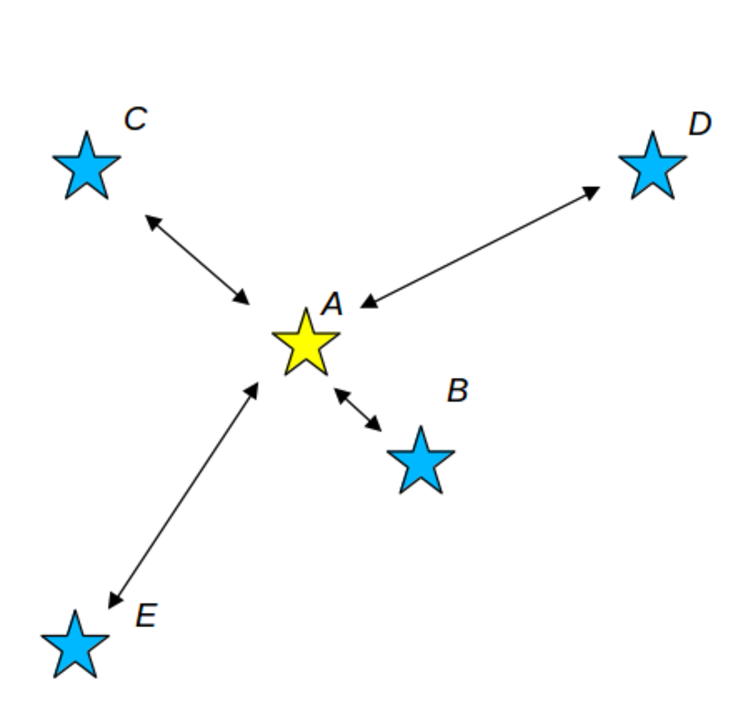
\includegraphics[width=\linewidth/3]{Figures/voting.png}
  \caption{Voting Eample.}
  \label{fig:voting}
  \end{center} 
\end{figure}

\begin{table}[H]
	\centering
	\caption{Voting Algorithm Example}
	\begin{tabular}{|l|l|l|l|l|}
		\hline
		\rowcolor{CU_Gold}
		\textcolor{white}{Observed Objects} & 
		\textcolor{white}{Measured Distance} & 
		\textcolor{white}{Reference Distance(s)} & 
		\textcolor{white}{Reference IDs} &
		\textcolor{white}{ID Votes}  \\ \hline
		A and B & $2.0^{\circ}$ & $1.9^{\circ}$ +- $.2^{\circ}$ 
		& 253 and 155 & 235, 155 \\ \hline
		A and C & $5.2^{\circ}$ & $5.15^{\circ}$ +- $.2^{\circ}$ 
		& 155 and 399 & 253, 155 (x2), 399 \\ \hline		
		A and D & $11.1^{\circ}$ & $10.93^{\circ}$ +- $.2^{\circ}$ 
		& 155 and 241 & 253 (x2), 155 (x3), 399 \\ 
		& & $11.24^{\circ}$ +- $.2^{\circ}$ 
		& 065 and 253 & 241, 065 \\ \hline
		A and E & $13.0^{\circ}$ & $13.1^{\circ}$ +- $.2^{\circ}$ 
		& 155 and 477 & 253 (x2), 155 (x4), 399 \\
		& & & & 241, 065, 477 \\ \hline	
	\end{tabular}
	\label{tab:voting} \\
\end{table} 

\noindent For images with point source beacons, if the ``unkonwn'' object is within the proximity of the beacon initial estimate, then it is considered a positive match for the beacon. For ``resolved'' beacons, there is no similar process as there should be less ambiguity over identifying resolved bodies due to an overall less number of objects due to the brightness and size of the beacon.\\
\\
Future work could further refine this process by adding additional validations steps as described in \cite{votingalgorithm}.

\newpage
\section{Tests}

\subsection{Test 1: Object ID Algorithm with Perfect Pixel Line Center Locations}
\textbf{Description}: This test verifies the object ID algorithm when the ``measured'' pixel-line coordinates for each object in the camera field of view matches perfectly the reference catalog positions. \\
\textbf{Methods}: objectIDStars(), pixelLineToEhat(), pixelLineToAngularSeparation(), generateUniqueIDAndCounts(), catalogIDsToRaDec() in objectIDFunctions.py\\
\textbf{Results}: \\
The perfect reference catalog IDs used as the object ID observed values are shown as ``Ref ID'' while the calculated IDs from the object ID algorithm are shown as ``Obj ID''. This test case passes as they both match perfectly.
\begin{figure}[H]
  \begin{center}
  \includegraphics[width=\linewidth/2]{Figures/objID_test1.png}
  \caption{Test Case 1.}
  \label{fig:test1}
  \end{center} 
\end{figure}

\begin{thebibliography}{9}
\bibitem{votingalgorithm} 
Michael Kolomenkin, Sharon Polak, and Michael Lindenbaum. ``A Geometric Voting Algorithm for Star Trackers.'' 
\textit{IEEE Transactions on Aerospace and Electronic Systems}, vol. 44, no. 2, 2008.

\bibitem{voyageruranus} 
S.P. Synott, A.J. Donegan, J.E. Riedel, and J.A. Stuve. ``Interplanetary Optical Navigation: Voyager Uranus.'' Jet Propulsion Laboratory California Institute of Technology.
\end{thebibliography}


\end{document}
